\section{Moduler}
\label{sec:moduler}
\frnote{hvorfor deler vi det op i moduler?}

Moduler i dette afsnit defineres som logisk grupperede funktionaliteter og modeller i løsningen. Hvert modul skal være uafhængig af andre moduler, og kun have et enkelt ansvar, og skal udelukkende håndtere sit eget ansvar. Et login modul skal derfor ikke have ansvaret, for at oprette en ny bruger. I stedet vil et dedikeret modul, til at oprette nye brugere, være favorabelt. Hvis hvert modul kun har et enkelt ansvar, kan moduler nemt genbruges i andre sammenhænge, eller udskiftes efter behov.

Modulerne i løsningen er beskrevet ved modulets funktionalitet, brugen af andre modeller og hvordan modellen overordnet er implementeret.

Kun de hidtil implementerede moduler er beskrevet i dette afsnit. I den fulde løsning, skal flere moduler implementeres, når funktionaliteten af løsningen skal øges. De beskrevne moduler er tænkt som en grobund for efterfølgende moduler.

\sinote{Diagram over alle moduler}

\subsection{Login}
\label{sub:database}

\kanote{mangler diagrammer og kodeeksempler}

Det første modul der interageres med, er login modulet, som har til formål at validere, og videresende brugeren til programmets hovedfunktioner. Login modulet har det primære ansvar for at angive adgangsniveauer, og sikre databeskyttelse. Fra login modulet kan man vælge at oprette sig som ny gæst, eller logge ind i systemet. Hvis brugeren vælger at oprette sig som ny gæst, så vil brugeren blive sendt til et separat modul.

Login modulet består af et standby- , medlemslogin-, validerings-, samt videresendings-element.

Standby-elementet er udgangspunktet for al interaktion med programmet, og har henvisninger til hvordan brugeren anvender programmet. 

Fra standby-elementet kan brugeren vælge at gå til medlemslogin-elementet, hvor en bruger der er medlem kan logge sig ind med sit medlemsnummer, og et kodeord.

Alternativt kan brugeren indsætte et chipkort fra standby-elementet, og så sender standby-elementet brugeren direkte til validerings-elementet.

Medlemsnummeret og kodeordet bliver videresendt til validerings-elementet, som krydstjekker informationerne via databasemodulet. Validerings-elementet videresender herefter en boolsk statusmelding, samt en brugerprofil fra databasen til videresendings-elementet.

Videresendings-elementet tjekker status meldingen. Hvis meldingen er falsk, sender den brugeren tilbage til enten medlemslogin eller standby, med en passende fejlmelding. Hvis valideringen gik godt, så videresendes brugeren til Hovedmodulet.
\subsection{Styringsmodulet}
\label{sub:styringsmodul}

Styringsmodulet har til opgave at instantiere og kontrollere de moduler som udgør specifikke funktionaliteter for brugeren.

\subsubsection{Funktionalitet}
\label{ssub:hovedmodul_funktionalitet}

Når en bruger har været igennem en succesfuld validering fra loginmodulet, bliver brugeren sendt videre til styringsmodulet. Dette modul fungerer som skelettet for de omkringliggende moduler. Brugeren bevæger sig derfor hele tiden rundt indenfor dette moduls rammer, indtil brugeren ønsker at forlade programmet. Da styringsmodulet ikke selv indeholder noget information direkte til brugeren, bør den altid instantiere et default element.

\subsubsection{Implementation}
\label{ssub:hovedmodul_implementation}

\begin{figure}
  \centering
  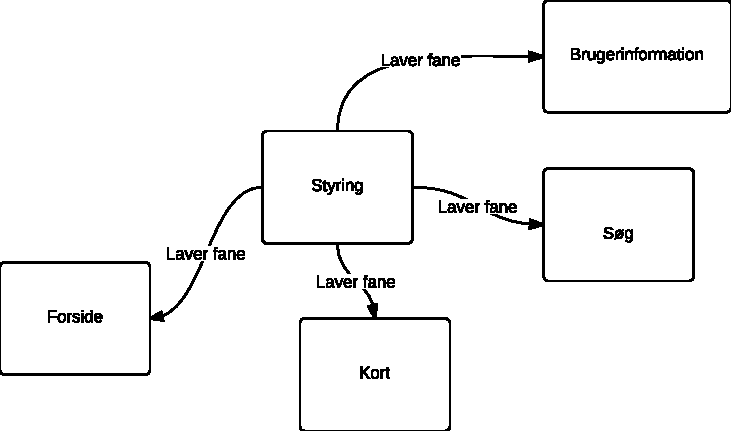
\includegraphics[width=\textwidth]{Main.pdf}
  \caption{Dette er bare noget filler tekst.}
\end{figure}


Styringsmodulet implementeres som en tabcontroller, der tilføjer andre moduler som faneblade. Default fanebladet er forsidemodulet. Dertil tilføjer styringsmodulet en kortfane, en brugerinformationsfane samt en søgningsfane. Disse faner bliver dog kun tilføjet, hvis brugeren, som er logget ind, har de nødvendige tilladelser. Når brugeren ønsker at forlade programmet, logges der ud, og brugeren sendes tilbage til loginmodulet.

\subsection{Persistenslag}
\label{sub:persistenslag}

\subsubsection{Funktionalitet}
\label{ssub:persistenslag_funktionalitet}

Persistenslag modulet har til opgave at manipulere og læse data fra en datastruktur. En datastruktur kunne f.eks. være en database eller en anden fil på harddisken. modulet tilbyder basale CRUD (create, read, update og delete) operationer, hvorfra alle tænkelige persistenslagsoperationer kan opbygges af.

Et eksempel på brugen af persistenslag modulet, kunne være login modulet. Login modulet skal verificere om et indtastet brugernavn matcher et indtastet kodeord. Til dette kan login modulet tilgå databasen igennem persistenslagets read operation, og herfra arbejde videre på den fundne data.


\subsubsection{Iplementation}
\label{ssub:persistenslag_implementation}

\frnote{Et billede med lidt tekst}

Persistenslag modulet er opbygget således at selve datastrukturen der manipuleres og læses fra, kan ændres. Herved indkapsles tilgangen til datastrukturen på en sådan måde, at et program kan gå fra at benytte en xml fil som data lager, til at benytte en database uden at ødelægge anden eksisterende kode.

Dette implementeres ved at persistenslag modulet er bevidst om en konkret implementation af tilgangen til en datastruktur. Når et andet modul ønsker at lave en læse operation på persistenslag modulet, videredelegeres denne operation til den underliggende implementation af tilgangen til en datastruktur.

\subsection{Kort}
\label{sub:kort}

\subsubsection{Funktionalitet}
\label{ssub:Funktionalitet}

Kort modullet har til opgave at give et visuelt overblik over alle bådpladser der eksisterer på en havn. Kortet præsenterer bådpladsers status i form af en beskrivende farve. F.eks. er en rød bådplads en optaget bådplads. På samme måde er en grøn bådplads fri. Kortet er interaktivt forstået på den måde, at kortets informationer er spejlet fra virkeligheden. Det vil sige at når en bådplads markeres som fri af et andet modul, skifter denne bådplads sin beskrivende farve til grøn på kortet.

Når der klikkes på en bestemt bådplads på kortet, kan følgende scenarier ske afhængigt af hvilken bruger der klikker.

\begin{description}
  \item[Bruger ligger selv ved bådpladsen] Brugeren bliver sendt hen til et modul der viser oplysninger om brugeren.
  \item[Bruger er et medlem. Der ligger en anden bruger på pladsen] Hvis brugeren har adgang til at se oplysninger om andre brugere, bliver brugeren sendt hen til et modul der viser oplysninger om brugeren.
  \item[Bruger er en gæst uden en eksisterende plads. Pladsen er ledig.] Brugeren bliver sendt til et reservationsmodul.
  \item[Bruger er en gæst med en eksisterende plads. Pladsen er ledig.] Da brugeren allerede har en plads, spørges om brugeren vil flytte til den nye plads.
\end{description}

\subsubsection{Implementation}
\label{ssub:Implementation}

En bådplads på kortet har en reference til en bådplads i databasen. Når en bådplads i databasen ændrer status, notificeres kort modullet, som nu kan ændre det visuelle status.

\subsection{Pladsregistrering}
\label{sub:plads_registrering}

\subsubsection{Funktionalitet}
\label{ssub:plads_registrering_funktionalitet}

Pladsregistreringsmodulet har til opgave at videreformidle bådpladsers tilstand til modellen. Når en ændring detekteres af modulet af et separat sensormodul, skal pladsregistreringsmodulet fungere som en adapter og ændre modellen tilsvarende. En bådplads kan have følgende tilstande:

\begin{itemize}
  \item Ledig
  \item Optaget af gæst
  \item Optaget af medlem
\end{itemize}



\subsubsection{Implementation}
\label{ssub:plads_registrering_implementation}

Modulet skal være bevidst om samtlige bådpladser, således at alle bådpladser kan få detekteret ændringer i deres tilstand. 
Modulet skal kunne håndtere flere forskellige implementationer af sensorer, således at løsningen ikke er afhængig af én type sensor, men kan lade dem skifte uden komplikationer.

\subsection{Medlemsinformation}
\label{sub:Medlemsinformation}

Brugerinformationsmodulet har til opgave at kommunikere mellem brugeren og databasen.

\subsubsection{Funktionalitet}
\label{ssub:Medlemsinformation_funktionalitet}

Kommunikation mellem databasen og brugeren indebærer, at vise information omkring en bruger, modtage inputs fra brugeren samt læse fra og skrive i databasen. At læse fra databasen indebærer, at den relevante information bliver hentet fra databasen, og vist på en acceptabel måde. Når der skrives til databasen menes der, at brugerens input bliver gemt i databasen. 

\subsubsection{Implementation}
\label{ssub:Medlemsinformation_implementation}

For at implementere dette består Brugerinformationsmodulet af et båd-, medlem- og rejse-delmodul. Delmodulerne har hvert deres tilsvarende ansvarsområde og er designet til at kunne læse, tilføje, redigere eller slette data fra databasen ud fra brugerens input. Læsningen af data foregår ved at et delmodul viser dets data i de respektive tekstfelter. For at redigere eller tilføje data, bliver der benyttet popup vinduer. Ved sletning af data markeres det ønskede elementer og der klikkes på fjern-knappen.
Ved at bruge popup vinduer, kan brugeren lettere kan skelne mellem at læse data og skrive data.
